\chapter{Introduction}

\section{Background}
\label{sec:Background}

The Hippocratic oath is a fundamental principle that guides decisions and advancements in the medical profession. It motivates doctors and physicians to make ethical decisions to minimize patient harm. It also drives physicians to continuously improve practices to reduce surgical risks and complications. This principle has driven the discovery of minimally invasive surgery (MIS). \citep{FIS-2021}


Minimally invasive surgery has become the standard practice across surgical fields and is a rapidly growing division in the medical industry. One branch of this field is laparoscopy, which is used to perform advanced and complex surgical procedures. \citep{FIS-2021}

Laparoscopy is surgical approach where small incisions are made to allow insertion of specialized equipment into the patient’s body. The primary instrument is the laparoscope, which is typically paired with other thin rod equipment based on the operations demands.  Compared to traditional open surgery, laparoscopy offers advantages including faster recovery rates and reduced morbidity and patient discomfort, though it requires a steeper learning curve. These benefits translate to cost savings through shorter hospital stays and reduced analgesic requirements. \citep{AIP-2018}


The laparoscope is a fundamental instrument to laparoscopic surgery. It consists of a thin rod with a camera attached to it at an angle, called the viewing angle, which is inserted into the patient’s body. The captured footage is displayed in real-time to the surgical staff on a monitor. Based on the visible footage, the surgical staff make a diagnosis, perform procedures, and coordinate instrument positioning based on the visual feedback. \citep{FIS-2021} Figure \ref{fig:Viewing Angle} illustrates what the viewing angle is.

\begin{figure}[H]
    \centering
    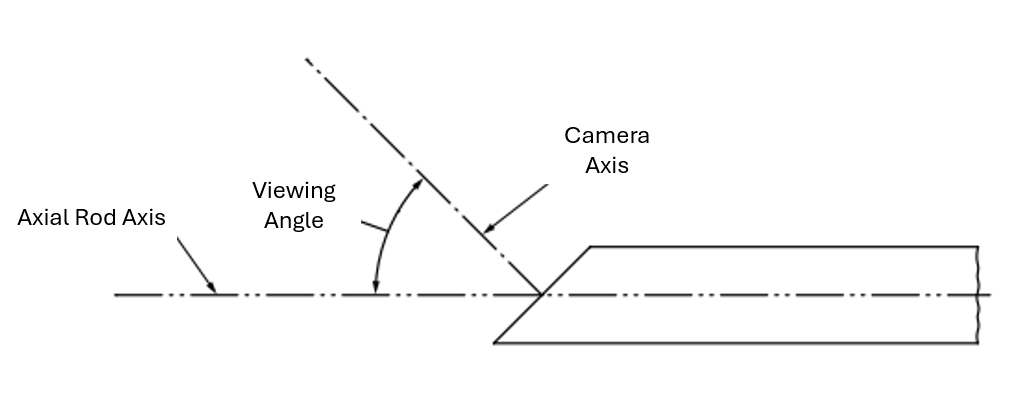
\includegraphics[height=4cm]{figs/Viewing Angle.png}
    \caption{Illustration of the viewing angle}
    \label{fig:Viewing Angle}
\end{figure}


Recent advancements in laparoscopy focus on improving the laparoscope’s visual capabilities through several approaches. These approaches include increasing the camera’s field of view, implementing three-dimensional (3D) visualization, and incorporating artificial intelligence (AI) or machine vision technologies to captured footage. Additional advancement made to modern laparoscopes is the utilization of robotic manipulators, with 3 or more degrees of freedom (DOF) to assist the doctor during operations. \citep{AIP-2018}


One of the main challenges of laparoscopic surgery is that it is a technically complex surgery to perform. Thus, inexperienced surgeons therefore require more training. However, laparoscopes are expensive equipment which makes them inaccessible for individual practitioners or small hospitals to purchase. \citep{JSE-2014} 

Additionally, Stellenbosch University host an open or career day, where potential students can attend to see which possible degrees they can study at the university. Ideally, the university would appreciate having a working laparoscope, to demonstrate how laparoscopic surgeries are performed. Consequently, the laparoscope will be used by the attending students to experience how laparoscopic surgeries are performed on phantom bodies.


Therefore, there is a need for a low-cost laparoscope, which will be used for training and demonstration purposes and not intended for use on living patients.


\section{Objectives}

The aim of this project is to design, build and test a low-cost laparoscope.

This project's main objectives are to:
\begin{itemize}
    \item Design, build and program a functional laparoscope by incorporating various Raspberry Pi components.
    \item Design a performance test to assess the laparoscope functionality and image quality abilities.
    \item Evaluate the developed laparoscope performance after performing the test.
\end{itemize}

\section{Scope}
\label{sec:Scope}

To develop the laparoscope, there are various aspects that need to be considered. These aspects range from physical properties to software properties and all have different scopes sizes. However, the scope for this project is subject to change based on the timeline of the project or change of the desired objectives of the project.

An important scope boundary is that the developed laparoscope, should not meet all medical grade standards. Since, it will not be used on living patients, the product should not be made out of medical grade equipment or materials. However, it needs to function similarly to medical grade laparoscopes, henceforth, should meet certain functionality standards for laparoscopic equipment.

Additionally, the developed laparoscope does not require having any degrees of freedom (DOF). The viewing angle, angle between the optical axis of the camera and the laparoscope axial axis, should aim to be 30 degrees. It is not required to incorporate a DOF to the viewing angle of the laparoscope.

To determine the laparoscopes capabilities and properties a testing station is required. Since Stellenbosch University does not have a testing station for laparoscopic products, it is required to design and build one, as well as articulate the testing procedures for the laparoscope. 

Considering the hardware components of the laparoscope, it is not within the project scope to manufacture hardware components from first principles. Rather, available hardware components will be purchased and repurposed if necessary to meet the project requirements. 

Considering software of the laparoscope, it is required that the system should be able to only operate the different modules. Any additional software application, such as machine learning or machine vision, is not within the project's scope. 



\section{Motivation}

As mentioned in Section \ref{sec:Background}, the main challenge with laparoscopic surgery is that it is a technically more complex procedure to perform, compared to open surgery. Thus, inexperienced surgeons require more training with the laparoscope and its additional equipment to achieve proficiency. However, laparoscopes are expensive surgical equipment, that isn't affordable investment for individuals or small medical facilities.


This project could also add value to the development of new medical robots. Most preliminary designs of medical robots require laparoscopes that can evaluate the robot's capabilities and flaws. However, they do not require expensive medically approved laparoscopes, rather, low-cost alternatives are preferable, as they minimize financial loss if damaged during testing or development. 

Additionally, a low-cost laparoscope can be used during future career days to demonstrate how laparoscopic surgeries can be performed for prospective students. 



\section{Use of AI Tools}

Anthropic is the main Artificial Intelligence (AI) company that will be used for this project, specifically its Claude Sonnet 4.5 model. This AI model assisted with research papers identification, sentence construction, grammar checks and code debugging. All AI-generated material will be reviewed and verified by the student to ensure the integrity and originality of the provided work. 

\section{Proposal Overview}

This report aims to enlighten the reader of the various sections of work performed to complete this project. Chapter \textit{\ref{sec:Literature Review}}  informs of the history of laparoscopy, afterwards it explains various segments of the work required to understand completing the project. Chapter \ref{sec:Design} aims to provide an overview of the design process for the laparoscope, while chapter \ref{sec:Heat} explains how a digital model was created of the laparoscope, to simulate how heat is transferred within the product. The following chapter \ref{sec:test} highlights all important test that were executed for the laparoscope. The last chapter of this report, chapter \textit{\ref{sec:Conclusion}}, provides a final motivation why this project was performed.

Additionally, in the appendixes, information is given regarding the scheduling of the project, the GA self-assessment, the planned work hours, and assembly drawings of the laparoscope.

